% !TEX root = ../foresight.tex

\section{Results}

In this section we provide experimental results that validate our approach.  A
video accompanies this submission and is available at \cite{foresight-video}.

\subsection{Localization Accuracy}

We tested our localization framework by emulating the car's UWB configuration inside a motion capture system. We placed motion capture
markers on the quadrotor and on each UWB sensor. This allowed us to
obtain the absolute position of the quadrotor and UWBs in the same coordinate
frame. We then flew the quadrotor inside the motion capture system and recorded
its predicted position determined by our localization and absolute position
using the motion capture markers. We ran 10 tests and were able to obtain an error of
13.7 cm, or 35.9\% the length of the quadrotor. Fig.~\ref{fig:localization}
shows how our localization compares to the ground truth. The green and red
lines respectively show the ground truth and predicted positions of the
quadrotor. While our accuracy is less than the system in \cite{tobiuwb}, the UWBs
in that study were all in the same plane. The accuracy of out-of-plane position estimation
using range measurements is lower than in-plane estimation because of the
larger state space. Since we wanted
our quadrotor to have the ability to fly beyond the plane of the roof-mounted UWBs,
we included additional out-of-plane UWBs which decrease accuracy compared to
having all UWBs in the same plane, but which help to provide greater accuracy for
out-of-plane measurements.


% \ja{How come it is worse than the reported errors in the UWB paper that we are citing?}

\begin{figure}

    \centering

    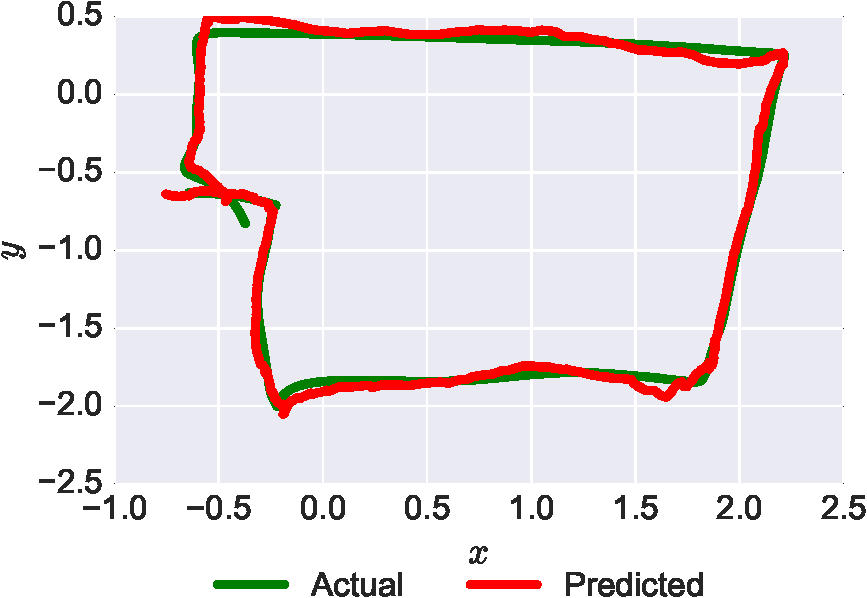
\includegraphics[width=0.5\linewidth]{localization}

    \caption{Comparison of our localization method with respect to
    ground truth. Ground truth was supplied by a motion capture system.}

    \label{fig:localization}

\end{figure}

\subsection{Experimental Setup}

For our experiments, we used a Toyota Prius with a SICK LMS1xx mounted on the
front of the car and six Decawave TREK1000 UWBs mounted on the
roof and front bumper of the car. A platform for the quadrotor to take off and
land was attached to the front bumper of the Prius. We used a Parrot Bebop 2
quadrotor with a Decawave TREK1000 mounted on the battery.  Fig.~\ref{fig:car}
shows the Toyota Prius and modified Bebop 2 quadrotor used in the experiments.

\begin{figure}[h!]

    \centering

    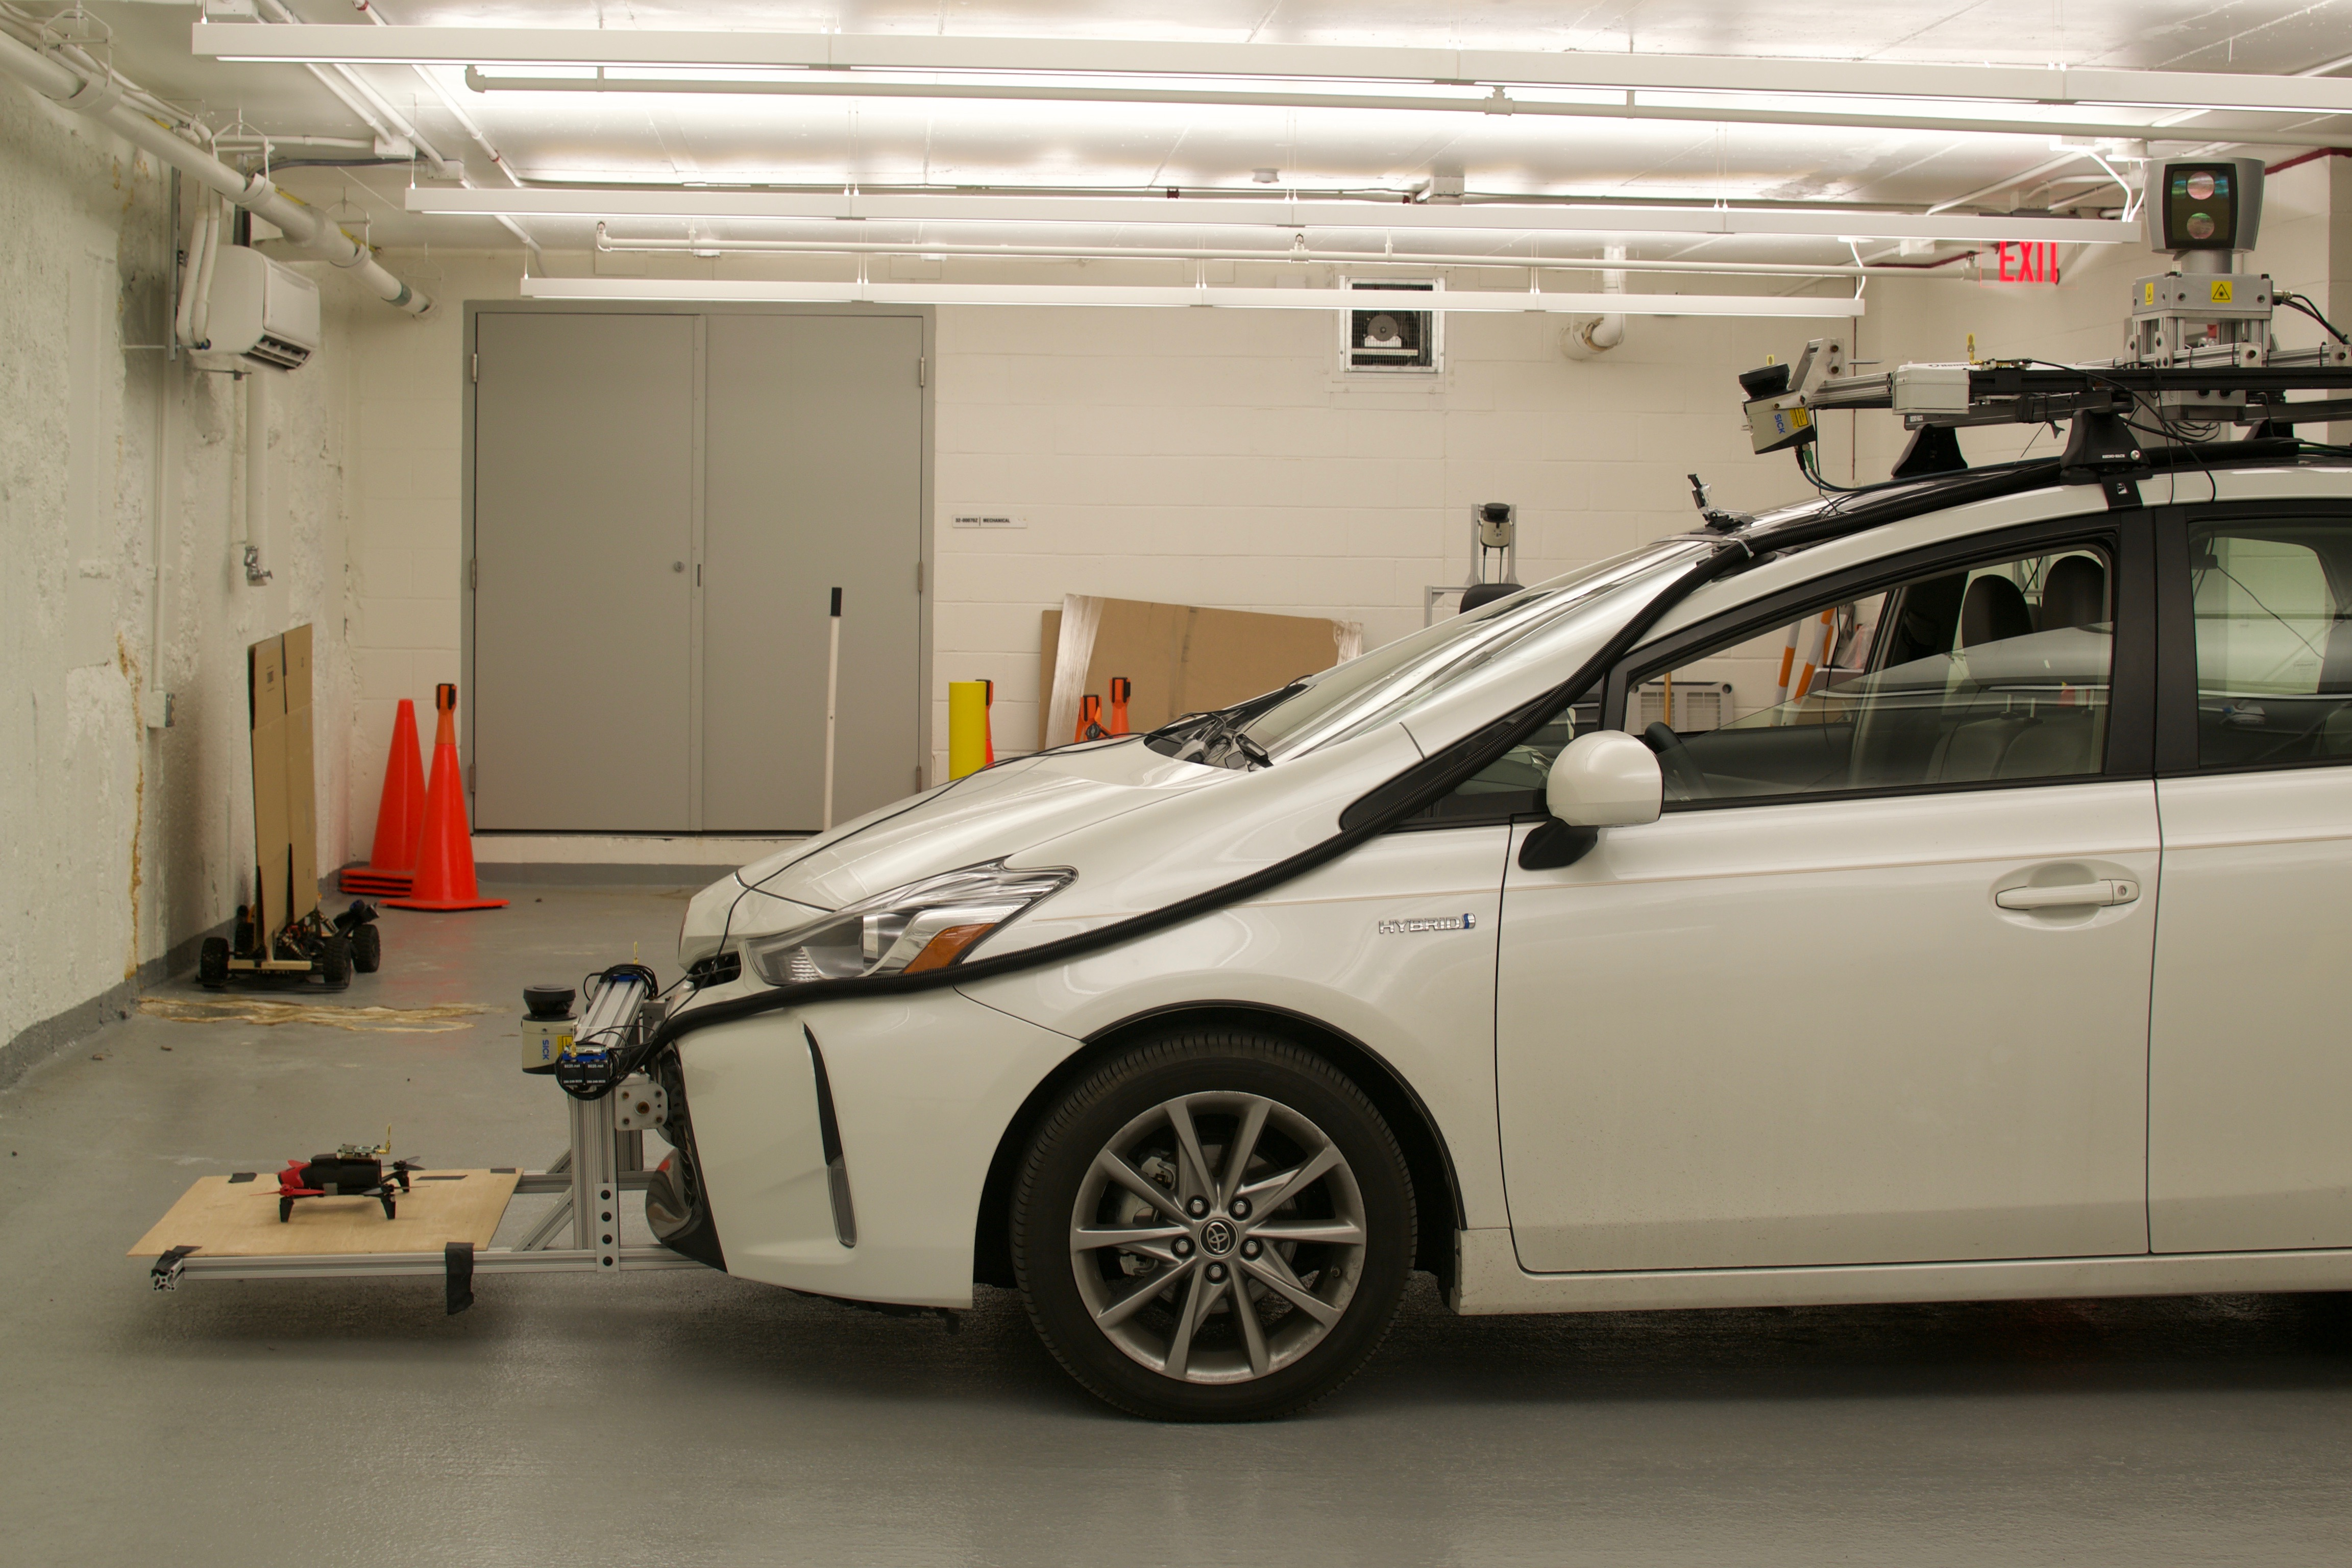
\includegraphics[width=0.49\linewidth]{car-side-view}
    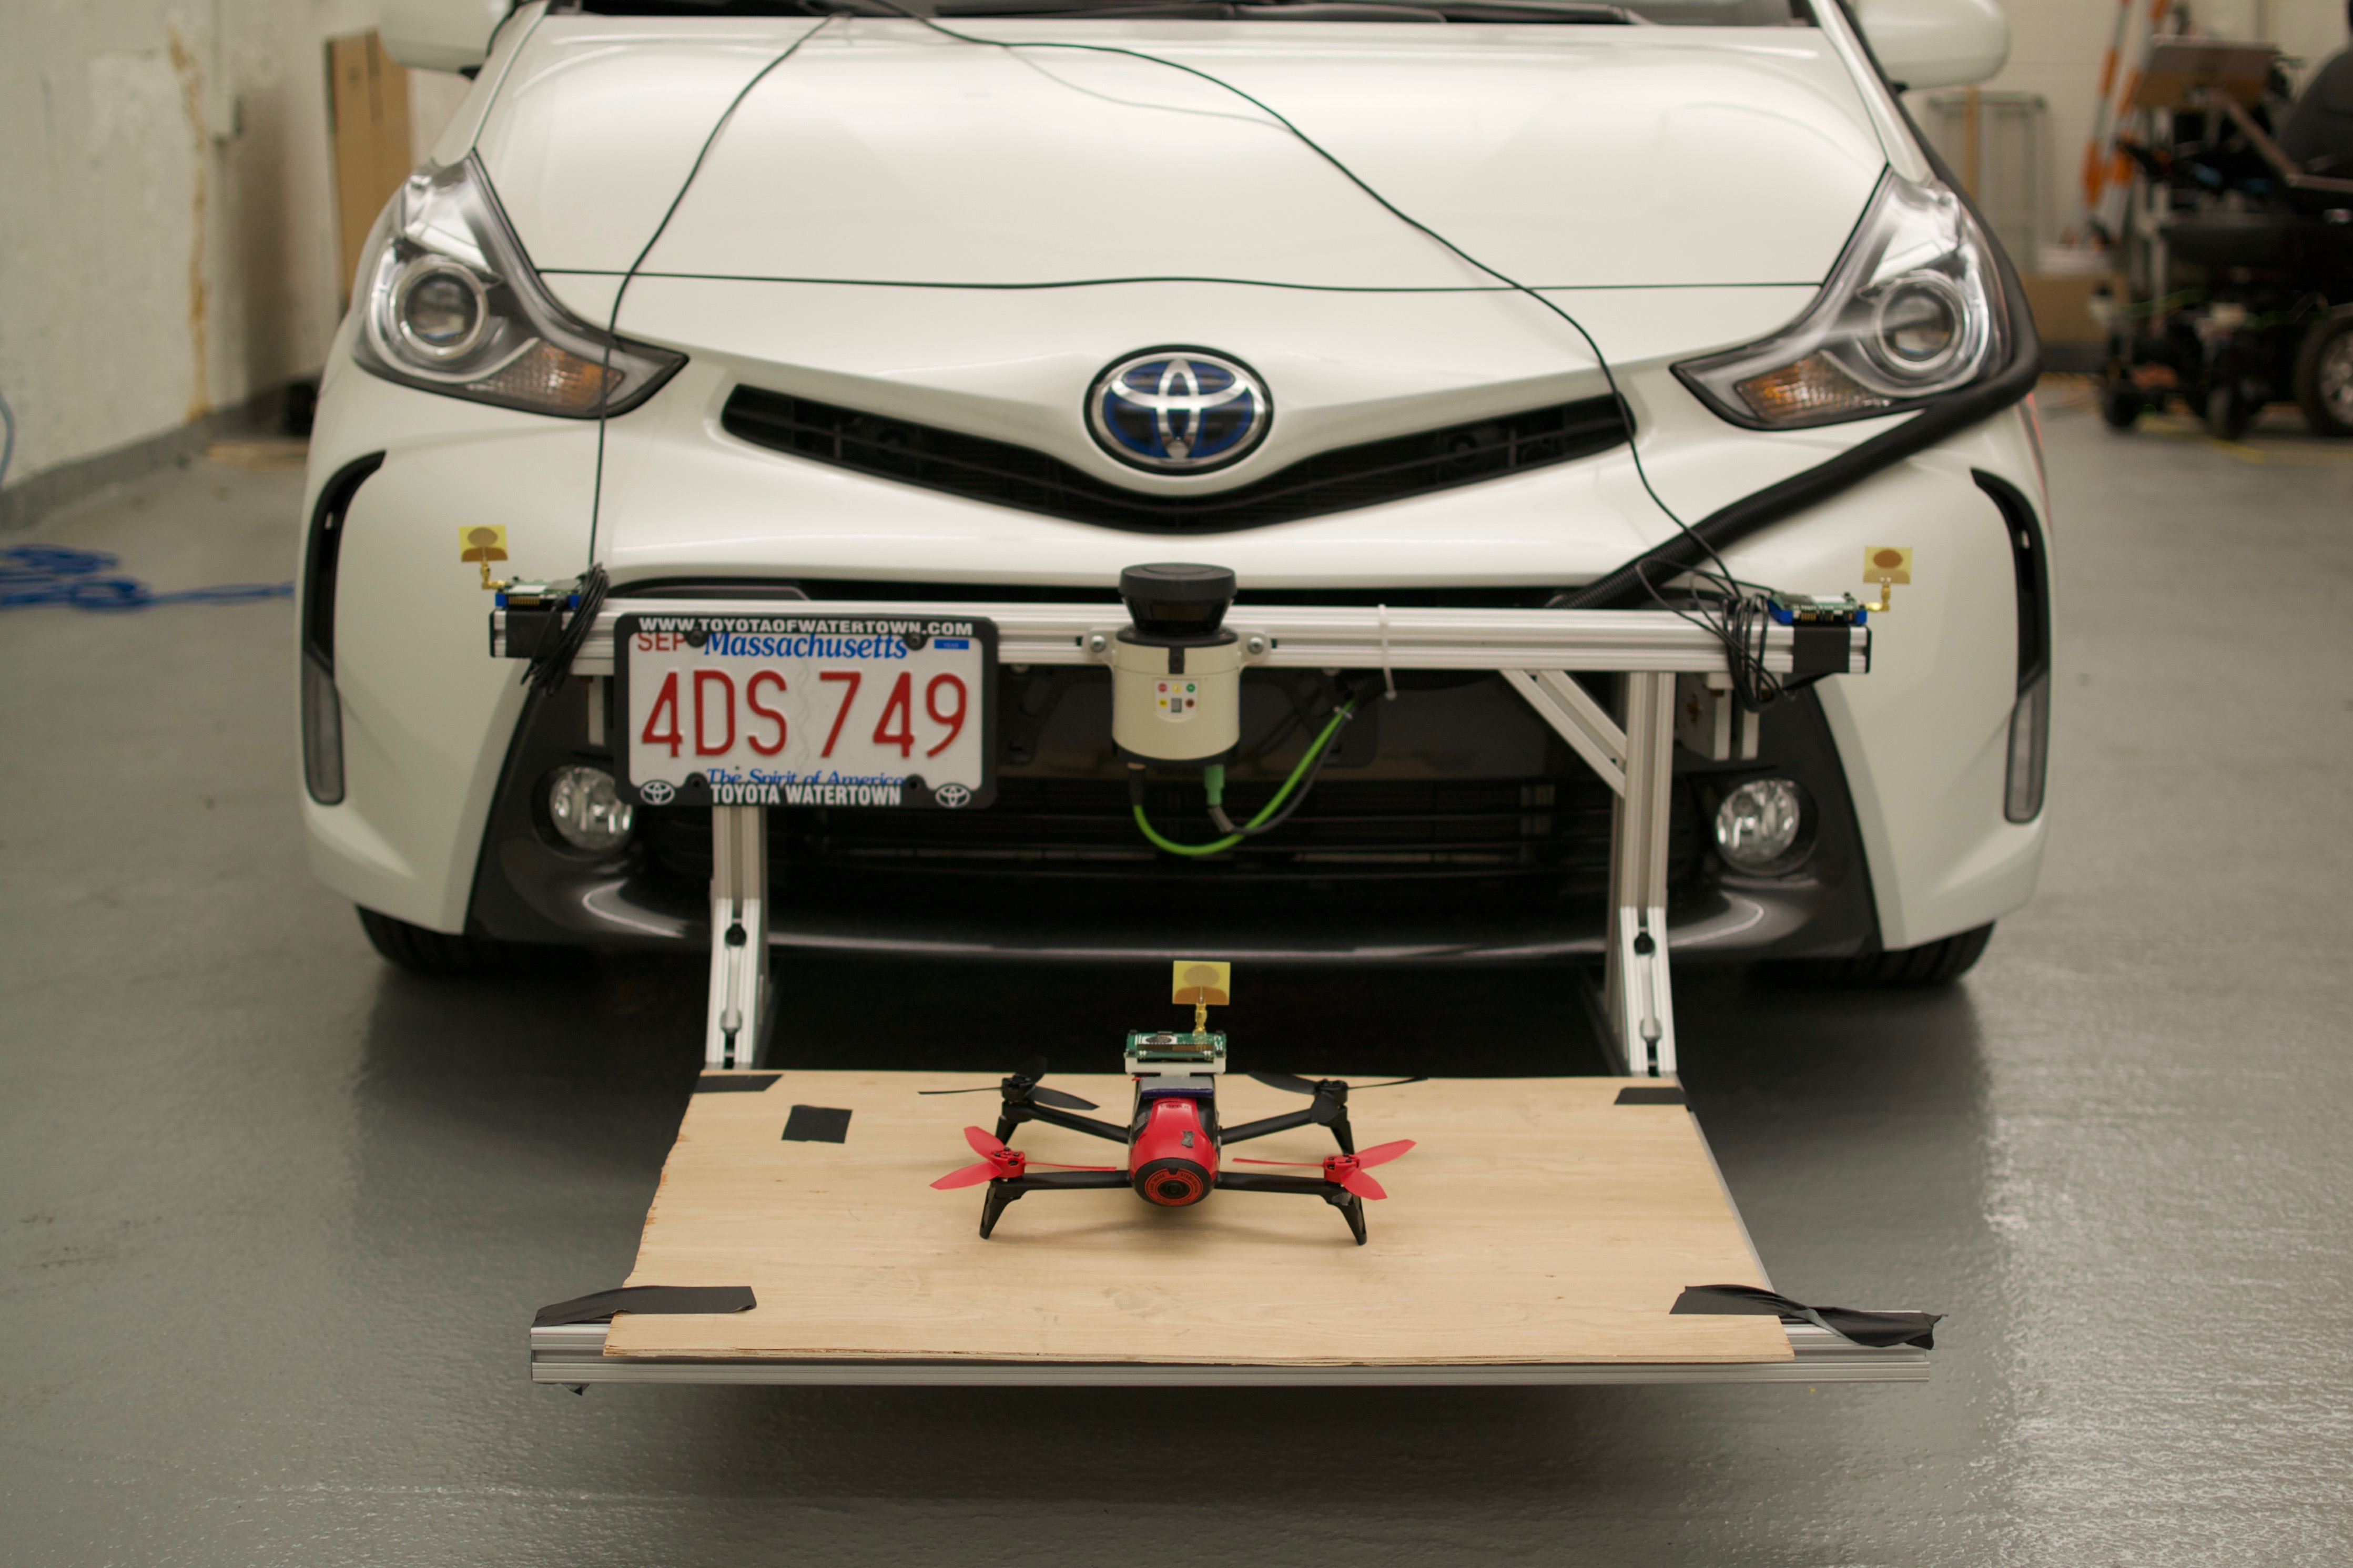
\includegraphics[width=0.49\linewidth]{car-close-up}

    \caption{Pictures showing Toyota Prius and Parrot Bebop 2 used in the
    experiments}

    \label{fig:car}

\end{figure}

We also ran tests using an autonomous golf cart as our ground vehicle in two
different settings.  One setting, shown in Fig.~\ref{fig:exp-buggy-inside}, was
artificially created using tall whiteboards as obstacles to mimic an
adversarial environment. The second, shown in Fig.~\ref{fig:exp-buggy-outside},
was a more realistic setting with the golf cart approaching an open garage door
with blind spots on either side. In both cases, the quadrotor was successfully
able to observe the blind spots and relay this information back to the computer
on board the golf cart. For the interest of brevity, we will only discuss in
detail the experiments using the Toyota Prius.

Our experimental scenario involves a car preparing to leave a garage with a
significant blind spot. The car is unable to sense around the corner to
determine if there are pedestrians or other cars that may obstruct its path.
Our quadrotor takes off from the car's front bumper platform and autonomously
flies out of the garage and looks around the corner. The car is then able to
leave the garage when there are no more pedestrians detected by the quadrotor.
Once the car is ready to return, it backs up into the garage. The quadrotor
then follows the car into the garage and autonomously lands on the platform.

\begin{figure}[t!]

    \centering

    \begin{subfigure}[t]{0.4\textwidth}

        \centering
        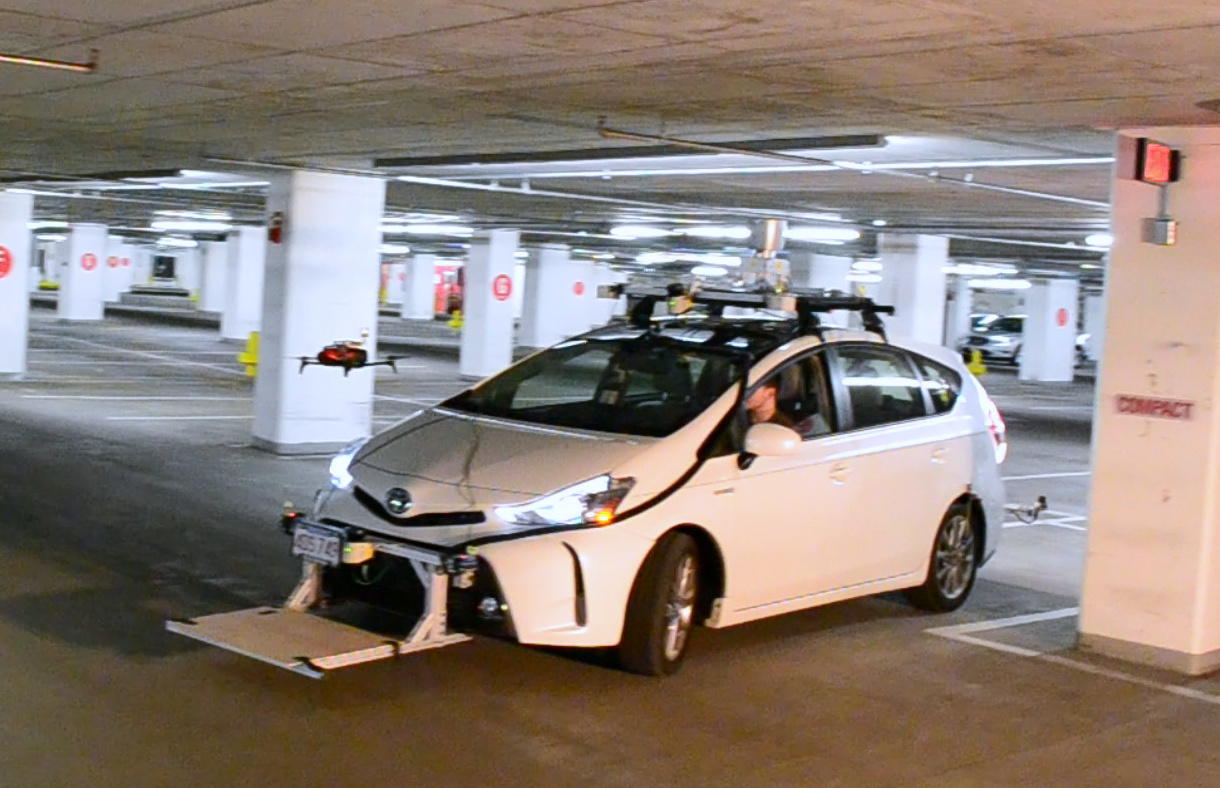
\includegraphics[height=1.1in]{exp-car-landing}
        \caption{}

        \label{fig:exp-car-landing}

    \end{subfigure}
    ~
    \begin{subfigure}[t]{0.4\textwidth}

        \centering
        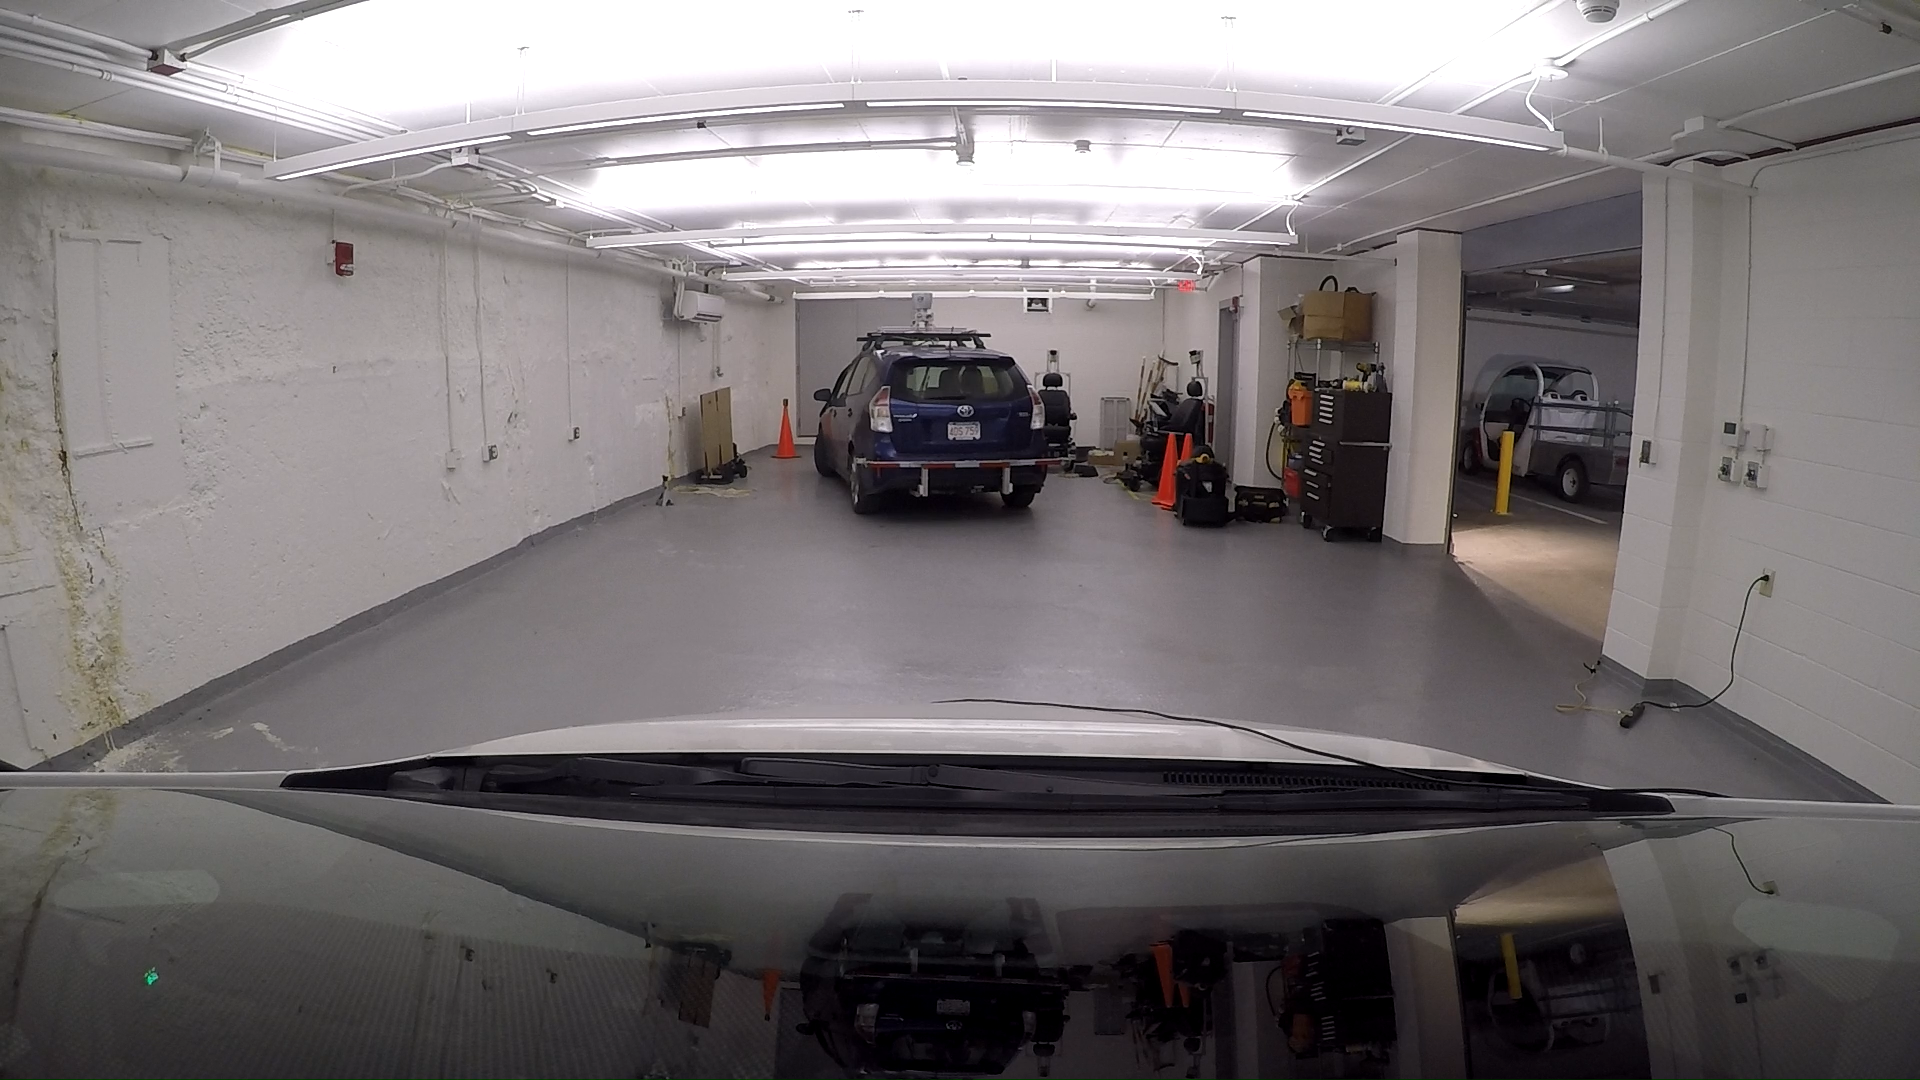
\includegraphics[height=1.1in]{exp-car-garage}
        \caption{}

        \label{fig:exp-car-garage}

    \end{subfigure}
    ~
    \begin{subfigure}[t]{0.4\textwidth}

        \centering
        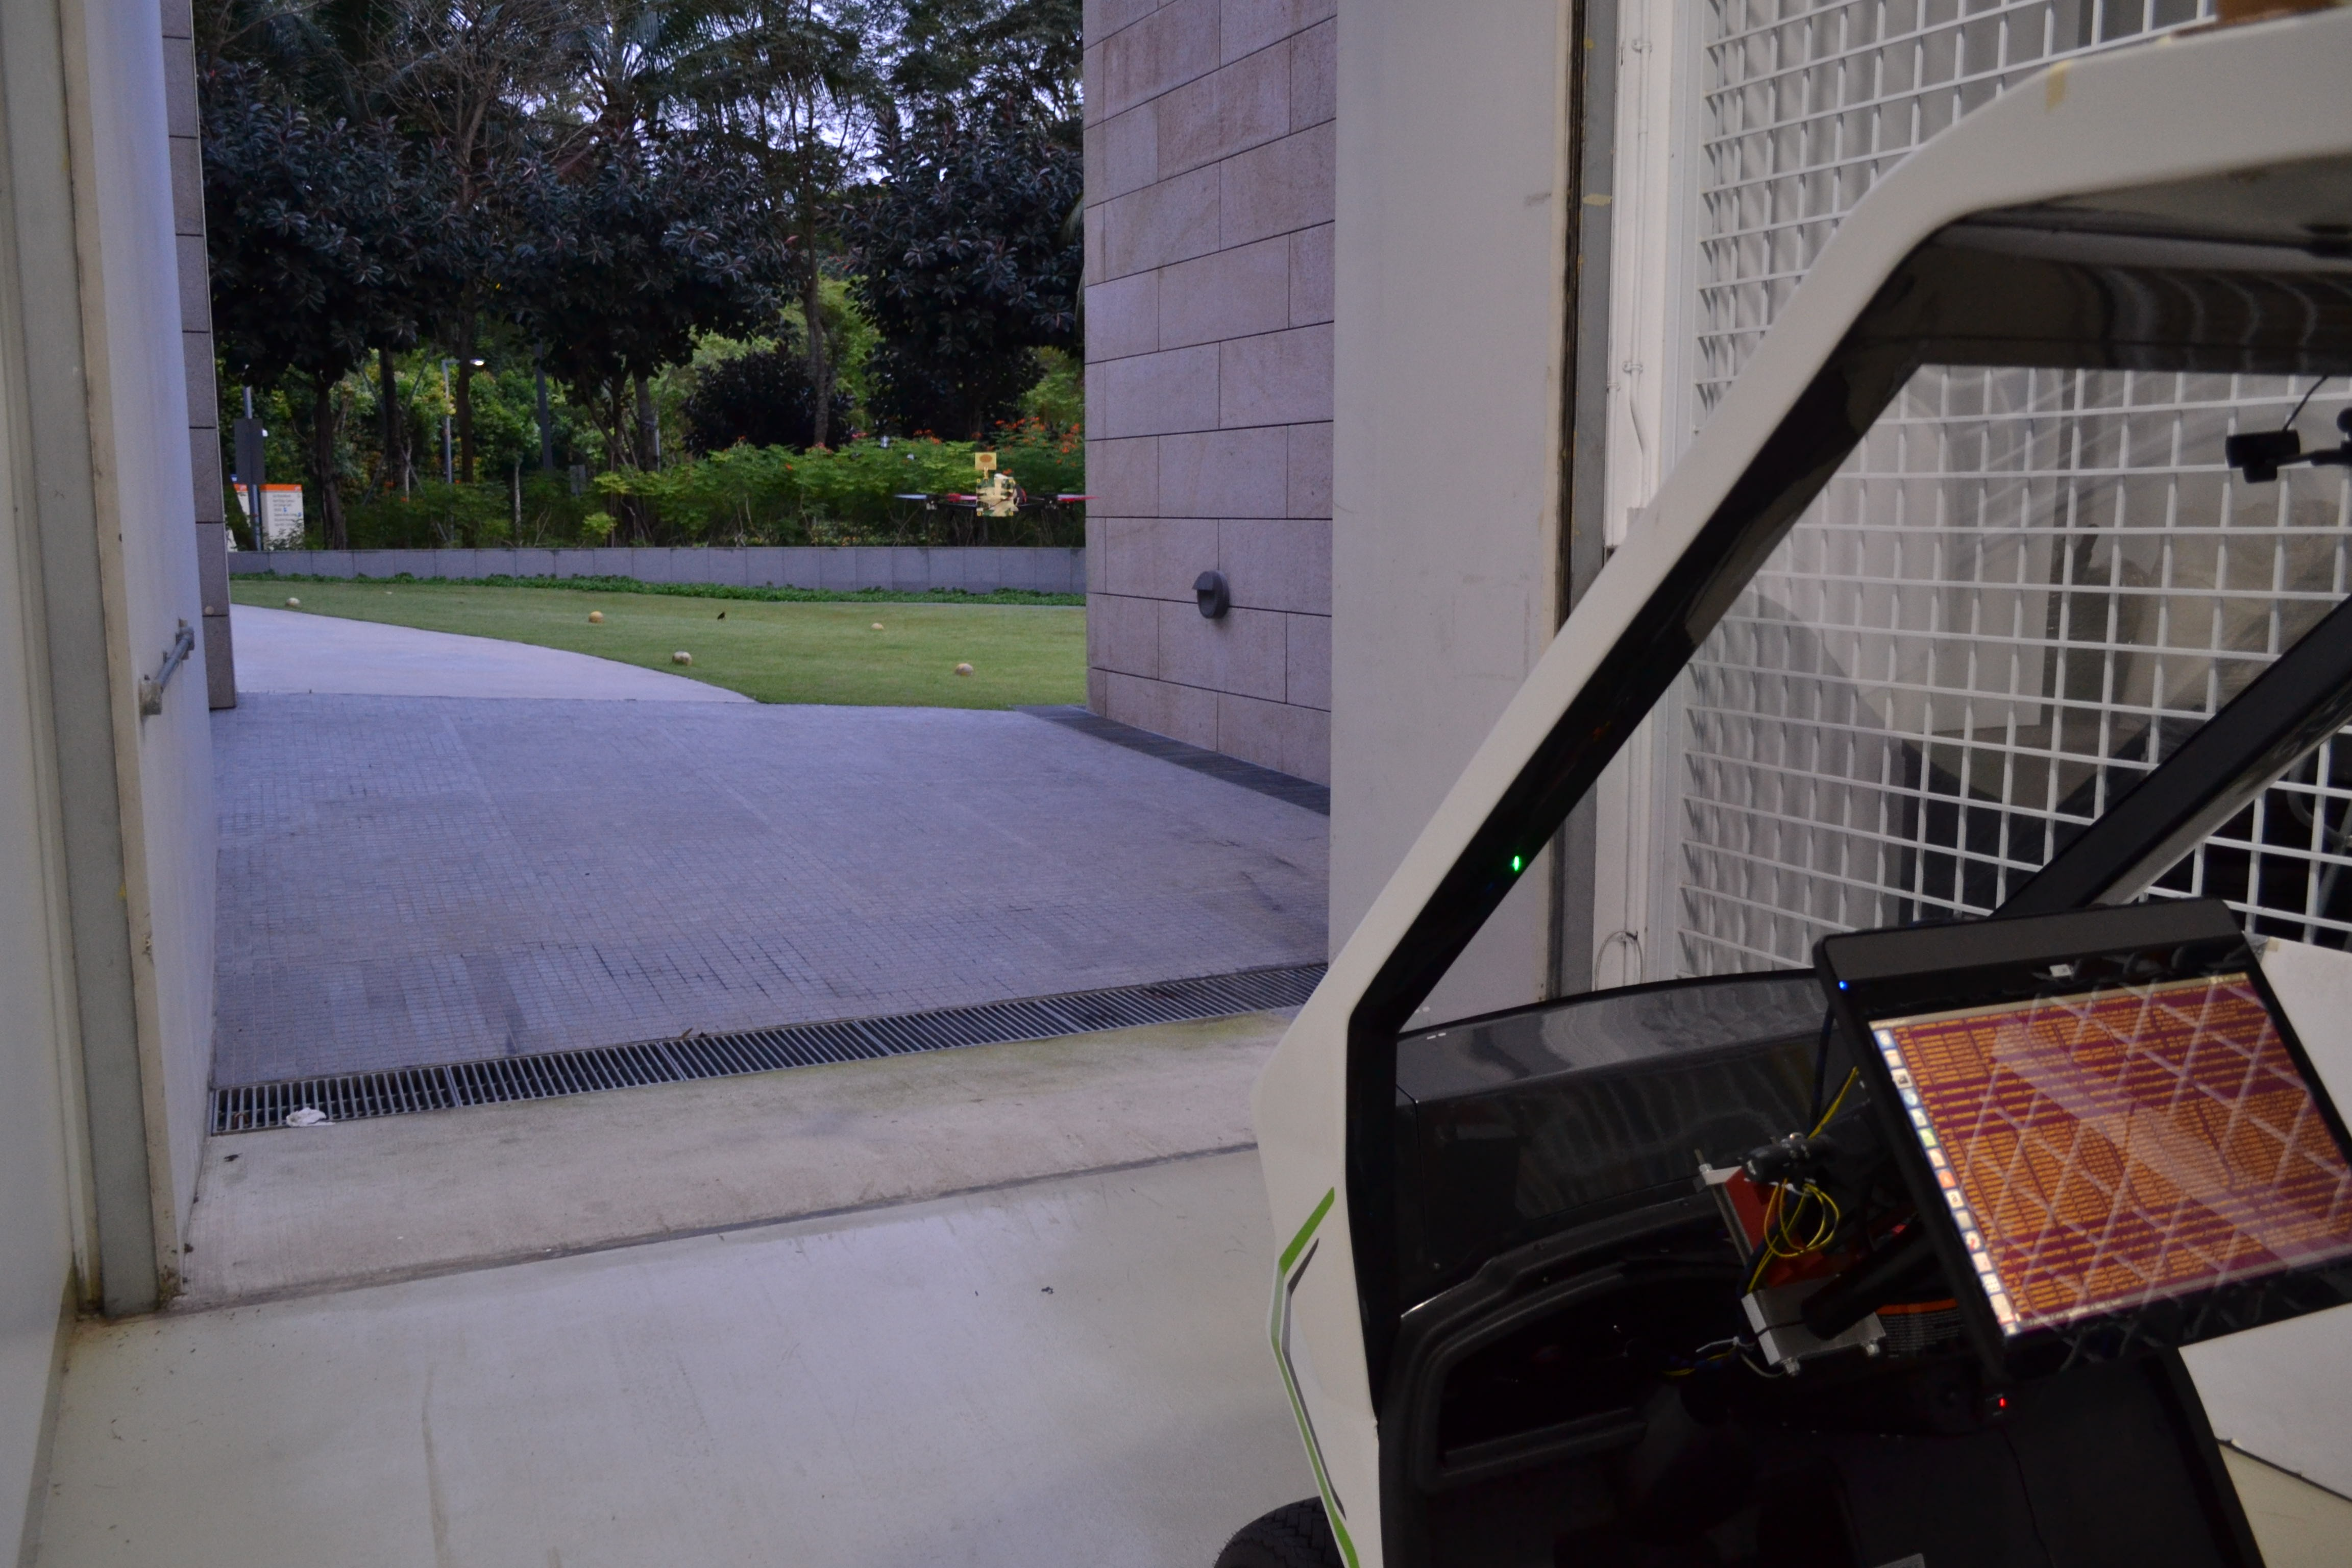
\includegraphics[height=1.1in]{exp-buggy-outside}
        \caption{}

        \label{fig:exp-buggy-outside}

    \end{subfigure}
    ~
    \begin{subfigure}[t]{0.4\textwidth}

        \centering
        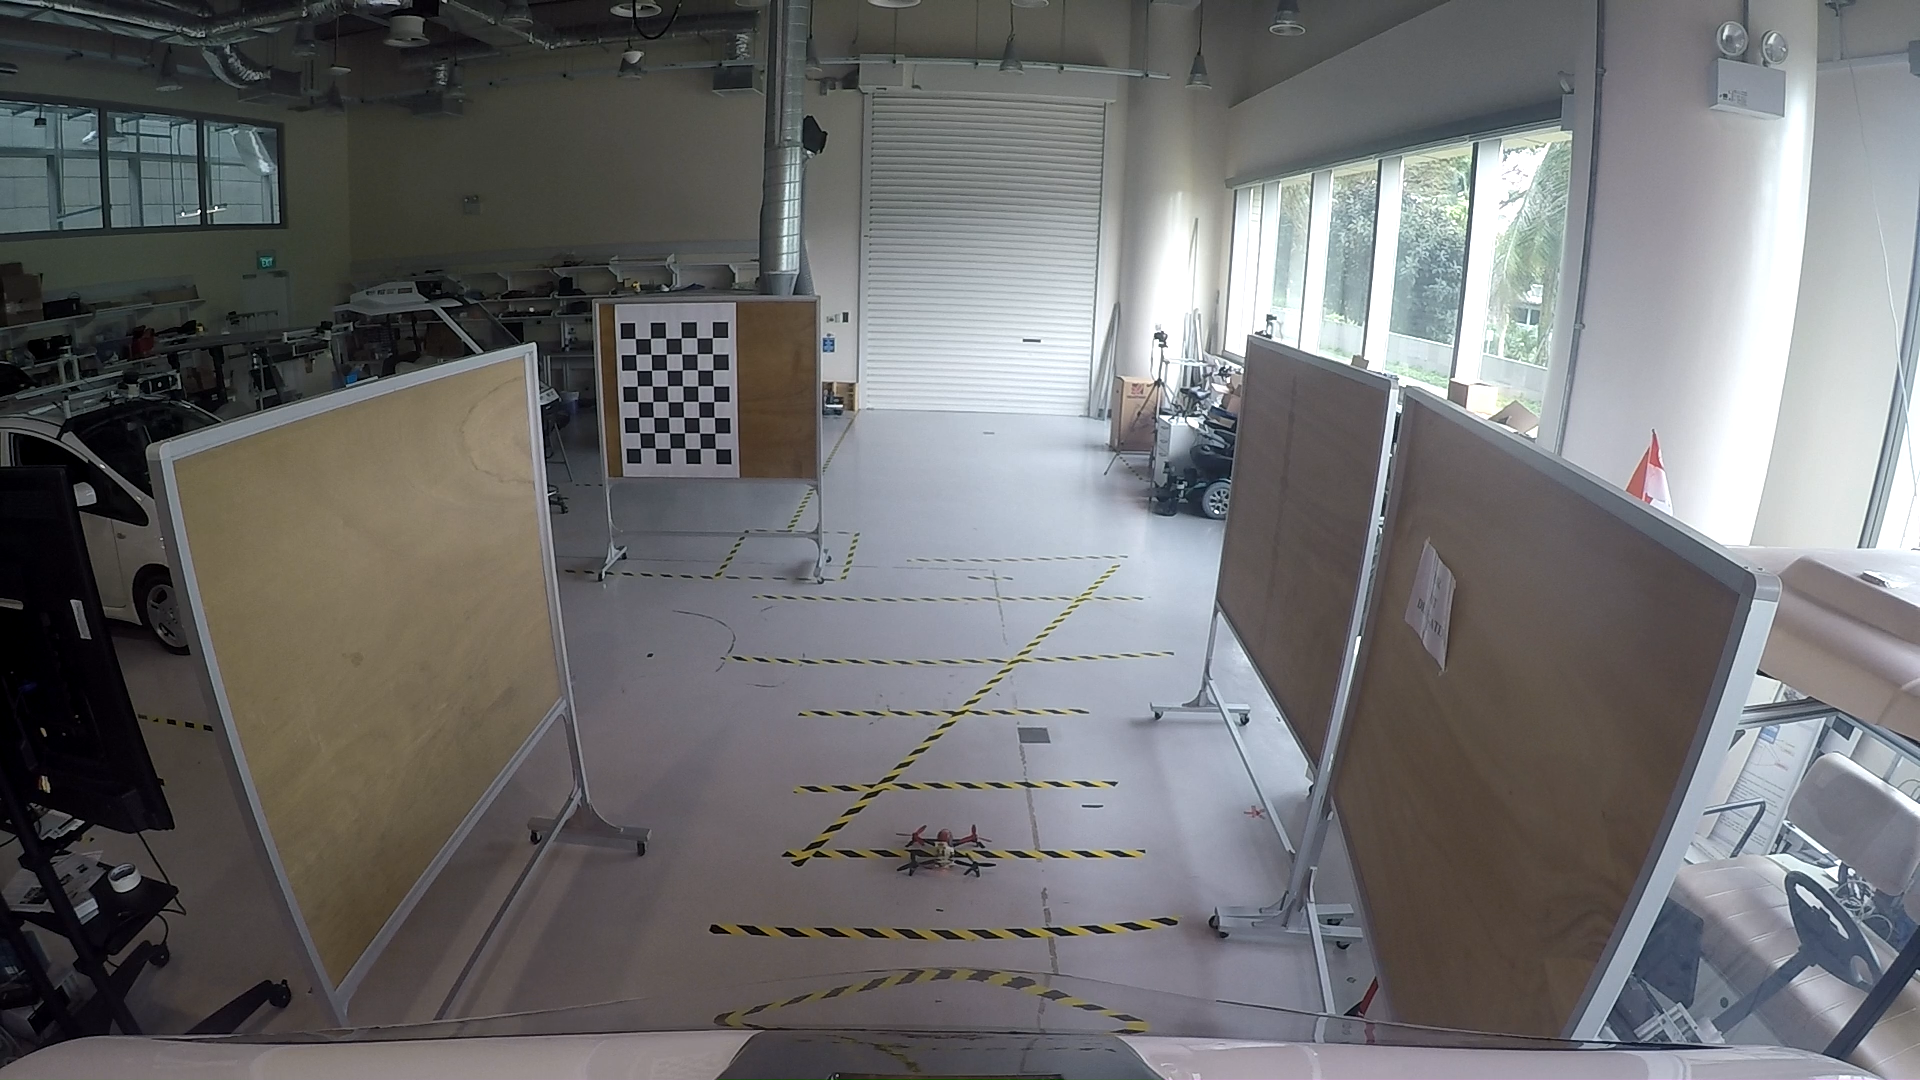
\includegraphics[height=1.1in]{exp-buggy-inside}
        \caption{}

        \label{fig:exp-buggy-inside}

    \end{subfigure}

    \caption{Snapshots from four experimental settings in which we tested our
    algorithm. Figures (a) and (b) used a Toyota Prius in a parking lot and a garage, respectively. Figures (c) and (d) used an autonomous golf cart in outdoor and indoor environments.}

    \label{fig:exps}

\end{figure}

\subsection{Experiment With Quadrotor}

Under each experimental condition shown in Fig.~\ref{fig:exps}, we conducted
multiple tests. In the course of one afternoon we performed 25 tests in the
environment shown in Fig.~\ref{fig:exp-car-garage} in which the quadrotor
successfully took off from the car, followed a path to observe blind spots, and
landed back on the car's platform. Each test took around a minute to
autonomously look around the corner and land back on the car. In every case,
take off, path following, and landing was successfully completed.  For the
remainder of this section we will detail one representative experiment.

% In addition, over 20 tests were conducted in the environment shown in
% Fig.~\ref{fig:exp-buggy-inside} and over 10 tests in
% Fig.~\ref{fig:exp-buggy-outside}.

\subsubsection{Looking Around the Corner}

Fig.~\ref{fig:experiment} shows snapshots of the experiment as it progressed.
The first column is a third person angle of the Prius and the quadrotor. The
second column shows frames from the quadrotor's on-board camera along with
object detection and classifications from the convolutional neural net. The
third column is a visualization of the sensor data from the car, the bounding
polygon, blind regions, and the quadrotor's plan. Each row shows a single
snapshot from the experiment.

The snapshots show that the quadrotor is able to successfully take off from the
car, use the laser scan to find the blind regions, and plan a path to look
around the corner in the garage. The last row shows that our system is able to
detect the pedestrian around the corner and provide the bounding box back to
the car.

Note that even though the quadrotor is not equipped with the sensors needed to
perform robust 3D obstacle avoidance, it is able to avoid collisions and fly
through the open garage door using the laser scan from the car.

\begin{figure}[h!]

    \centering

    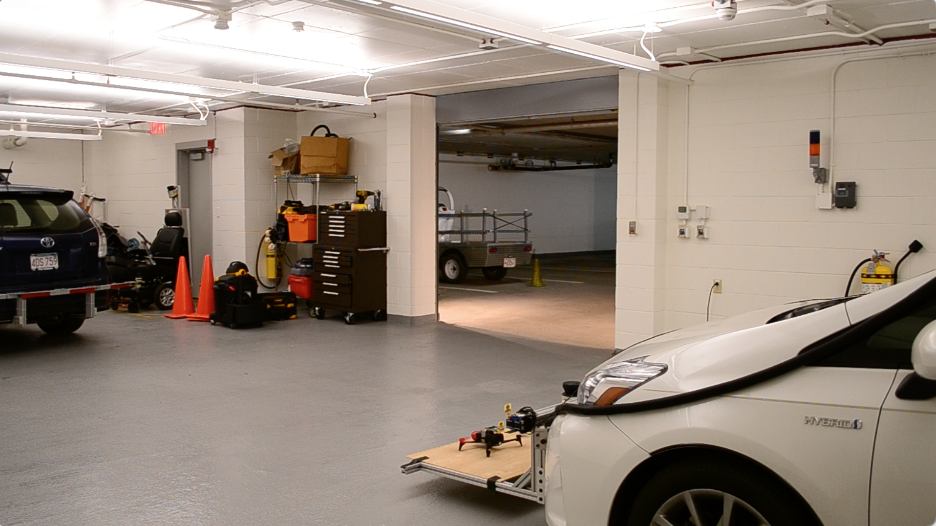
\includegraphics[width=0.35\linewidth]{00-third-person}
    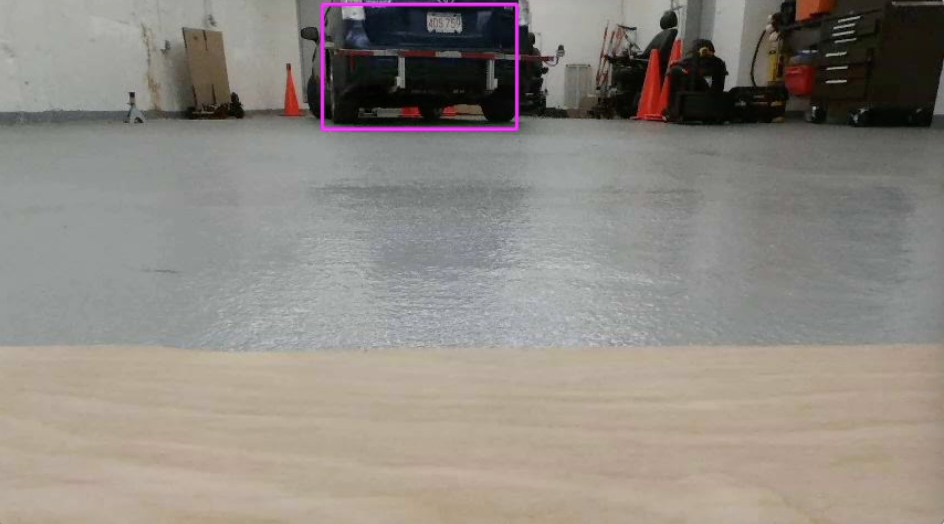
\includegraphics[width=0.35\linewidth]{00-quad-cam}
    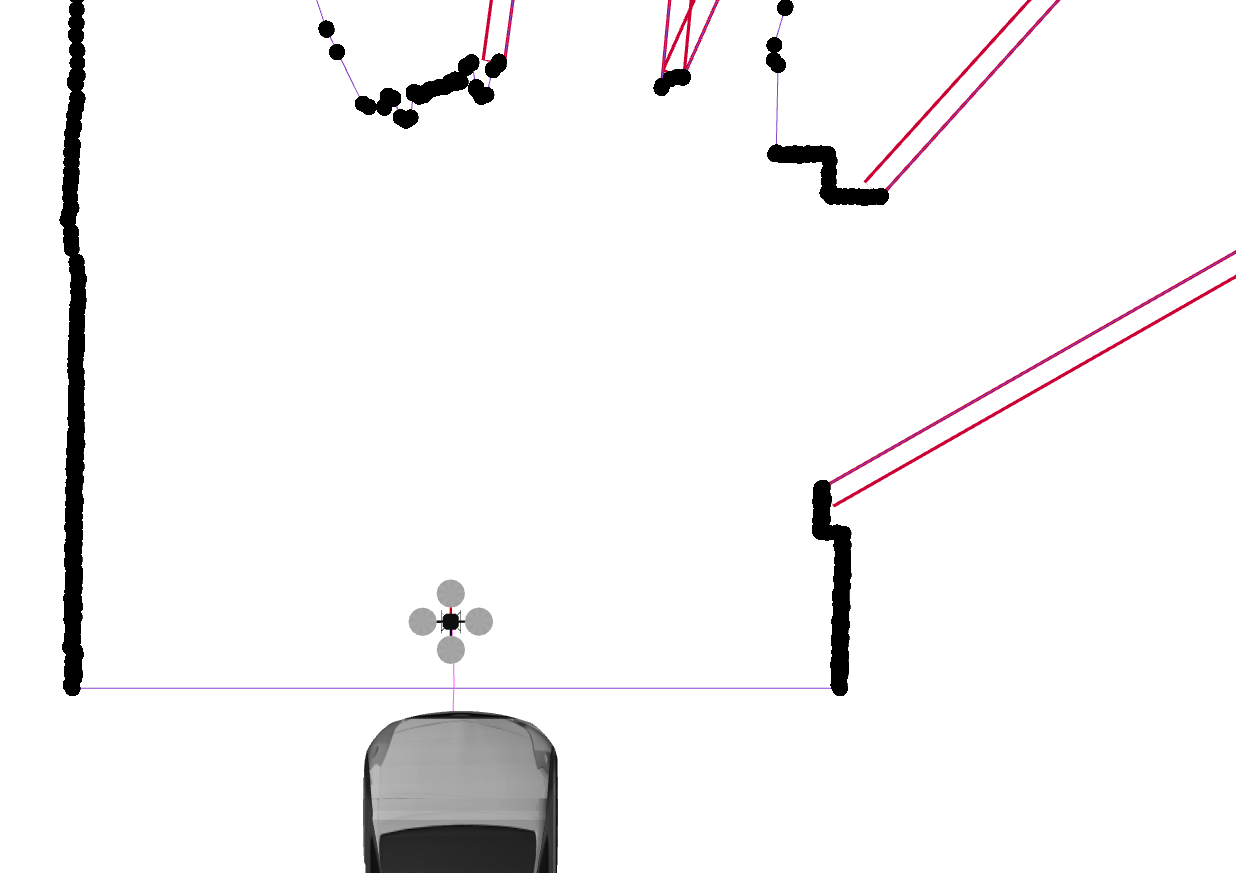
\includegraphics[width=0.28\linewidth]{00-planner-step} \\
    \vspace*{1mm}
    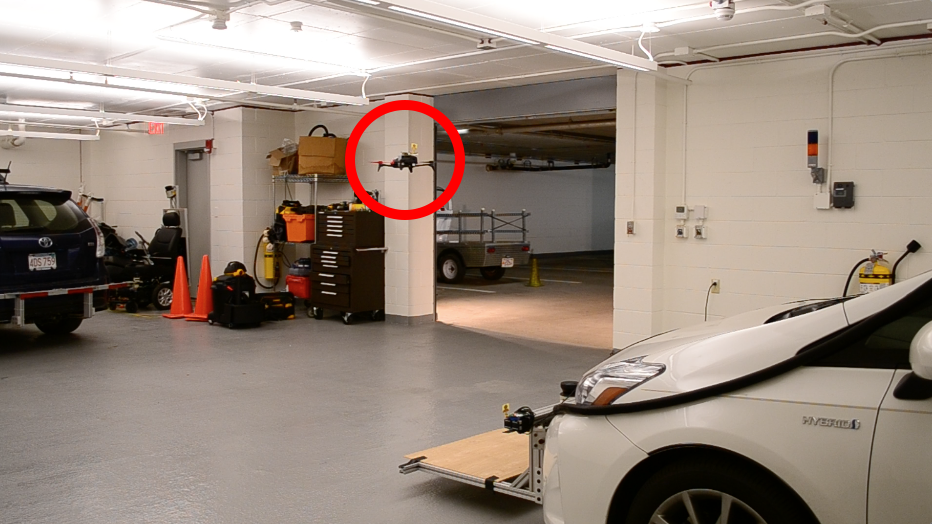
\includegraphics[width=0.35\linewidth]{01-third-person}
    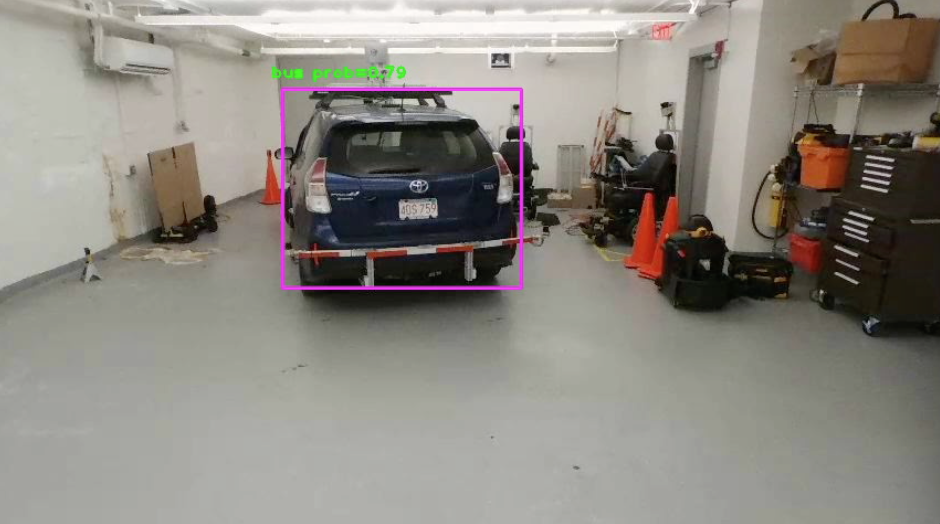
\includegraphics[width=0.35\linewidth]{01-quad-cam}
    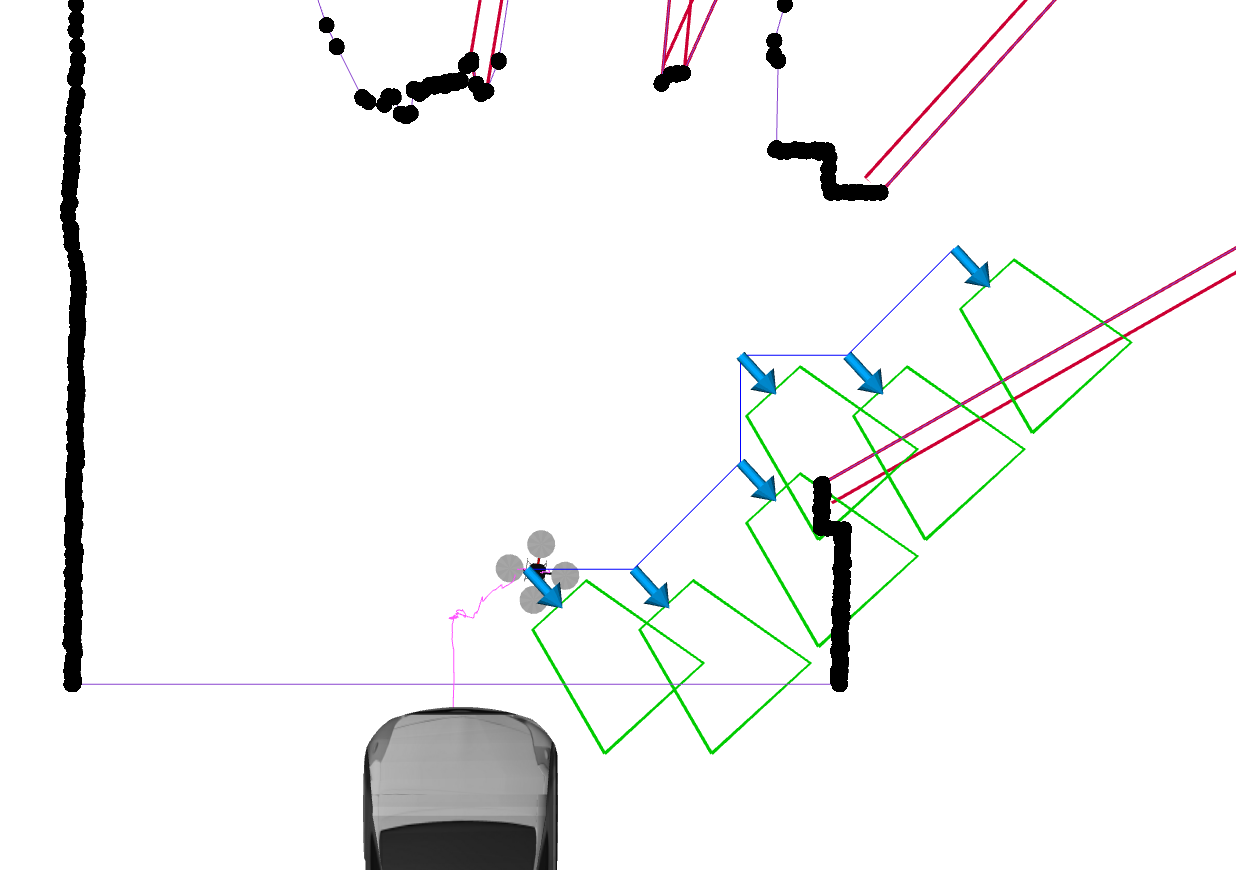
\includegraphics[width=0.28\linewidth]{01-planner-step} \\
    \vspace*{1mm}
    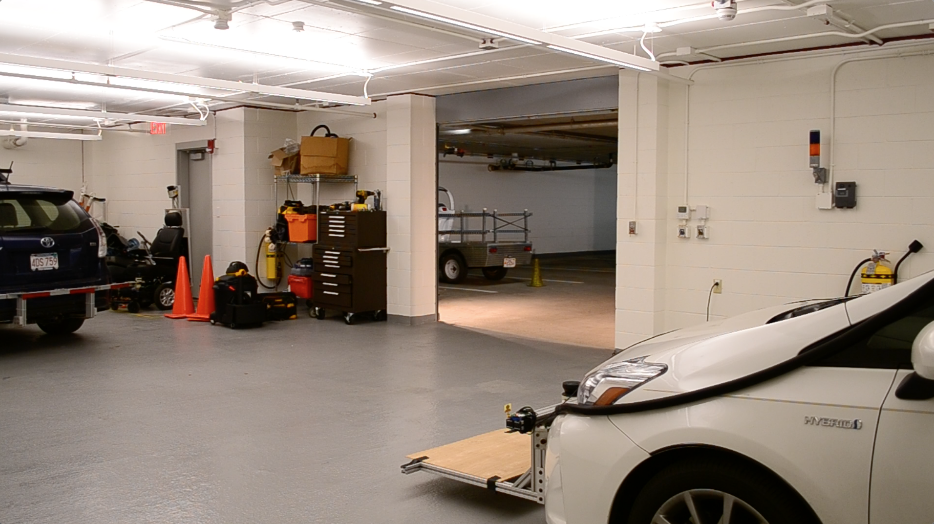
\includegraphics[width=0.35\linewidth]{02-third-person}
    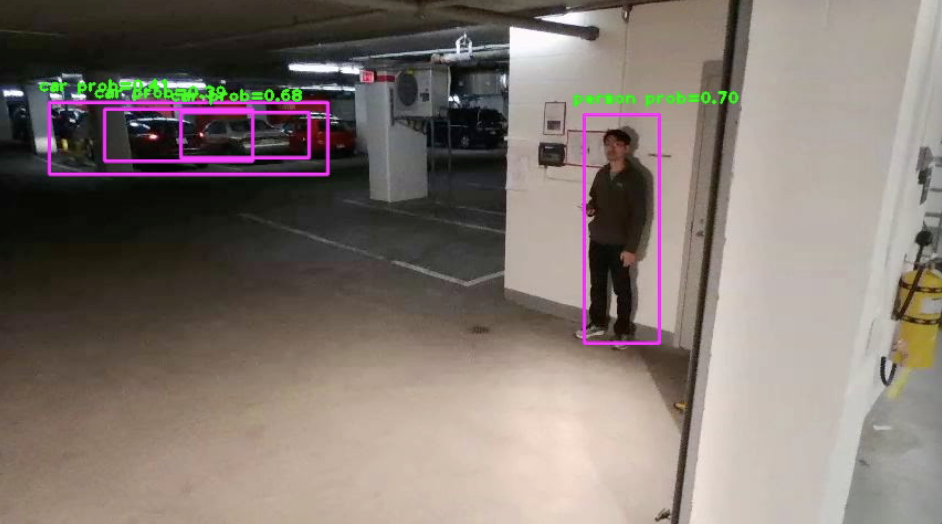
\includegraphics[width=0.35\linewidth]{02-quad-cam}
    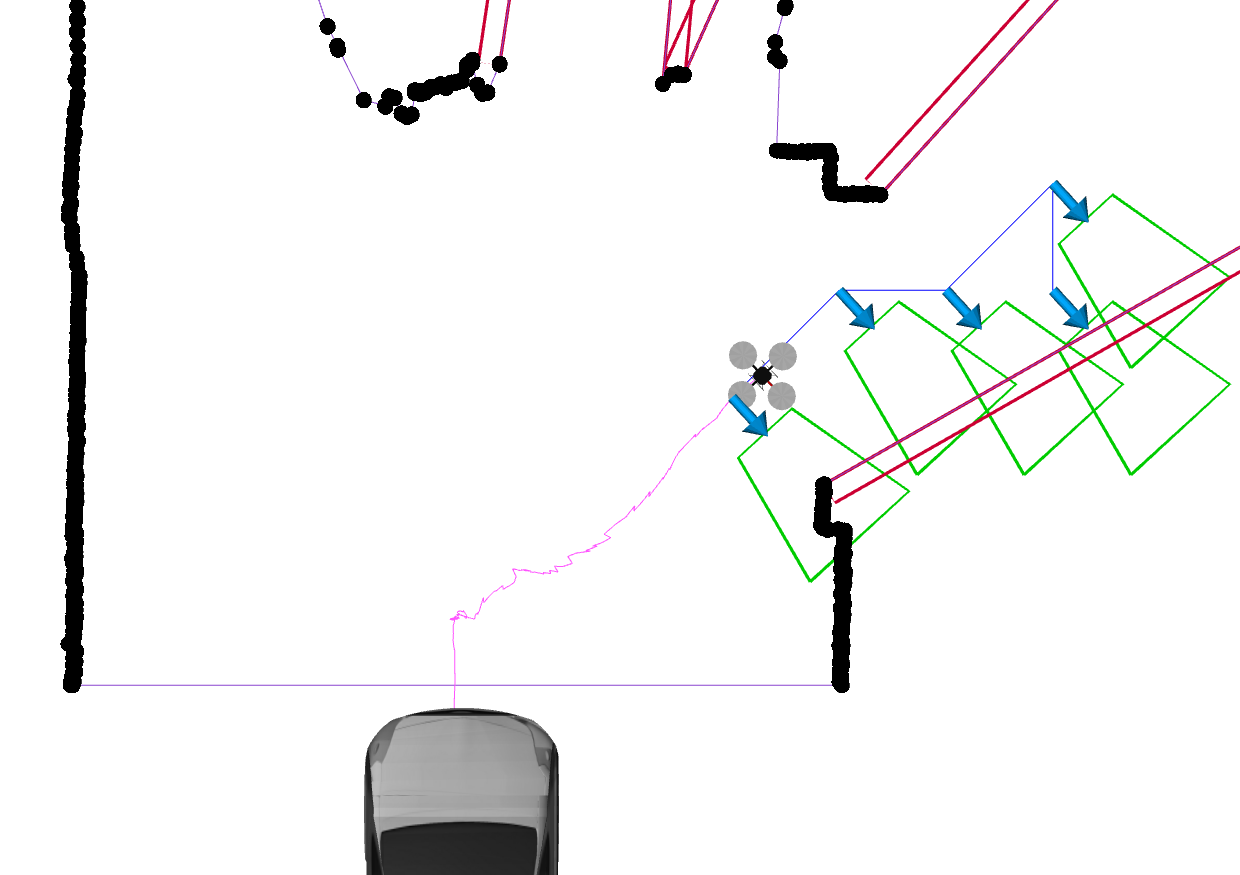
\includegraphics[width=0.28\linewidth]{02-planner-step}

    \caption{Snapshots from the experiment as it progressed. The second column
        is from the quadrotor's on board camera. The third column shows a
    visualization of the planner.}

    \label{fig:experiment}

\end{figure}

% Under each experimental condition shown in Fig.~\ref{fig:exps}, we conducted
% multiple tests. Over 20 tests were conducted in the environments depicted in
% Fig.~\ref{fig:exp-car-garage} and~\ref{fig:exp-buggy-inside}. Over 10 tests
% were conducted in the environment shown in Fig.~\ref{fig:exp-buggy-outside}.

\subsubsection{Landing On the Car}

Once the car is ready to park, the quadrotor is able to autonomously land back
on the platform attached to the front bumper. Fig.~\ref{fig:landing} shows
snapshots from the experiment as the quadrotor followed the car and landed on
the platform. The first image in Fig.~\ref{fig:landing} shows the quadrotor
following the car as it backs up into a garage. The second shows the car parked
and the quadrotor hovering over the platform. The last image shows the
quadrotor after it successfully landed on the platform.

\begin{figure}[h!]

    \centering

    \centerline{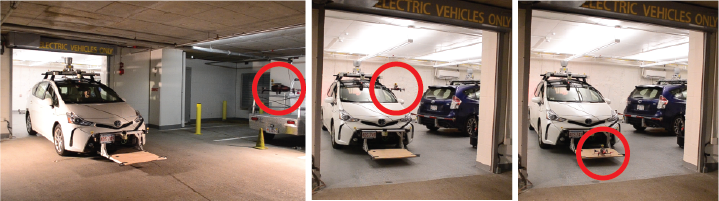
\includegraphics[width=1\linewidth]{landing_sequence}}

    \caption{Snapshots of the quadrotor landing on the car}

    \label{fig:landing}

\end{figure}
